\begin{figure}[H]
\centering
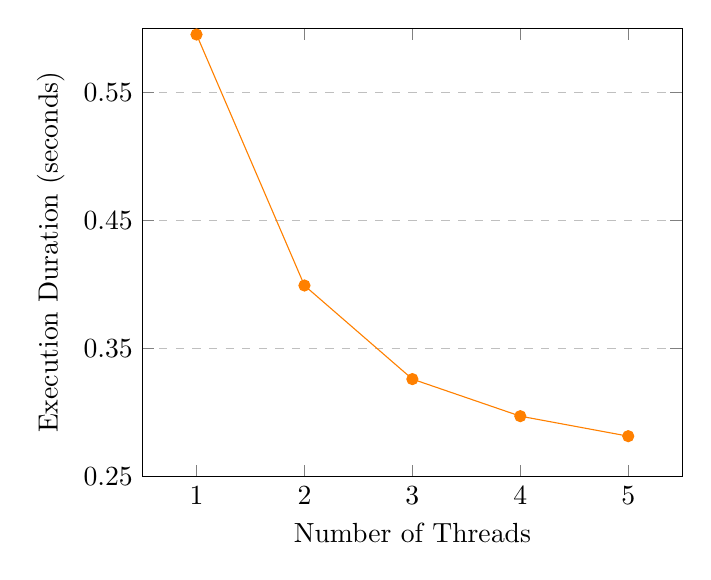
\begin{tikzpicture}
\begin{axis}[
    xlabel={Number of Threads},
    ylabel={Execution Duration (seconds)},
    xmin=0.5, xmax=5.5,
    ymin=0.25, ymax=0.6,
    xtick={1, 2, 3, 4, 5},
    ytick={0.25, 0.35, 0.45, 0.55, 0.65},
    ymajorgrids=true,
    grid style=dashed,
]
\addplot[
    color=orange,
    mark=*,
    ]
    coordinates {
    (1,0.595073778) (2,0.399138181) (3,0.326064784) (4,0.297126143) (5,0.281510981)
    };

\end{axis}
\end{tikzpicture}
\caption{Execution Duration vs. Number of Threads for Birch3}
\label{fig:birch}
\end{figure}